\documentclass[12pt]{memoir}

\def\nsemestre {V}
\def\nterm {Verano}
\def\nyear {2021}
\def\nprofesor {Adri\'an Barquero}
\def\nsigla {MA0609}
\def\nsiglahead {T\'opicos en Teor\'ia de N\'umeros}
\def\darktheme {}
\input{../../../headerVarillyDiff}

\begin{document}
%\clearpage
\maketitle
%\thispagestyle{empty}
{\small
\setlength{\parindent}{0em}
\setlength{\parskip}{1em}

La teoría de curvas elípticas tiene al día de hoy más de 50 años de ser desarrollada continuamente. Fermat estudió ecuaciones que tenían relación  con curvas elípticas y es hasta el día de hoy que se pueden ver las relaciones con estos temas. Este tema se puede ver desde las distintas areas de la matemática: análisis, álgebra, geometría... Hay métodos para el uso de firmas digitales y seguridad en tarjetas de crédito que están relacionados con curvas elípticas.\par
En fín, este tema es de mucho interés en la actualidad. Nosotros nos centraremos en los números racionales siguiendo la línea del libro de Silverman \& Tate \cite{SilvermanTate}. En concreto los temas a tratar son los siguientes:
\begin{enumerate}
  \item Introducción a geometría proyectiva.
  \item Curvas cúbicas y ecuaciones en forma normal de Weierstrass.
  \item Suma de puntos y la ley de grupo en curvas elípticas.
  \item Puntos de orden finito y el teorema Nagell-Lutz.
  \item La estructura del grupo de puntos racionales en una curva elíptica y el teorema Mordell-Weil.
\end{enumerate}


\subsubsection*{Requisitos}
Se asume un conocimiento básico de teoría de números. Se utilizarán conceptos de teoría de grupos y variable compleja a un nivel básico.
}
\newpage
\tableofcontents
%\begin{multicols}{2}

\chapter{Curvas elípticas}

\section{Día 1| 20210105}

\subsection{Introducción a la geometría proyectiva}

\subsubsection{La vista algebraica}

En general hay más de una manera en la que uno puede construir el plano proyectivo y más generalmente el espacio proyectivo en varias dimensiones. A manera de motivación, a la hora de estudiar ciertos problemas en matemática, se llega a observar que es suficiente trabajar con objetos en términos de clases de equivalencia.\par
Por ejemplo un problema que se discute en el Silverman y Tate \cite{SilvermanTate}, al estudiar las soluciones racionales de la ecuación
$$x^N+y^N=1,$$
se puede ver que si $x=\frac ac$ y $y=\frac bd$ son soluciones racionales en su forma más reducida ($\mcd(a,c)=\mcd(b,d)=1$, y $c,d>0$) entonces debe ocurrir que $c=d$. Esto se logra después de un breve análisis de divisibilidad. Concluimos que la solución debe tener la forma $x=\frac ac$ y $y=\frac bc$.\par
Esta solución satisface que $a^N+b^N=c^N$ por lo que la solución $\left(\frac ac,\frac bc\right)$ del problema en términos racionales genera una solución $(a,b,c)$ de la ecuación homogénea $x^N+y^N=z^N$. La clave aquí es que como la ecuación es homogénea, cualquier múltiplo de $(a,b,c)$ va a ser una solución al mismo problema. Pero como estas soluciones se obtienen de manera relativamente trivial, podríamos querer considerarlas como equivalentes. Este tipo de razonamiento lleva a la definición algebraica del plano proyectivo.

\begin{Def}
  El \term{plano proyectivo} sobre un cuerpo $K$ es el cociente del conjunto $\set{(a,b,c)\in K^3\less\set{(0,0,0)}}$ por la relación
  $$(a,b,c)\sim (a',b',c')\iff \exists t\in K^\x(a=ta',\ b=tb', c=tc').$$
  Denotamos entonces
  $$\bP^2_K=\quot{\set{x\in K^3\less\set{0}}}{\sim},$$
  y la clase de equivalencia de $(a,b,c)$ la denotamos $[a,b,c]$ y se llamarán sus coordenadas homogéneas.
\end{Def}

\begin{significant}
  ¿Qué pasa si incluimos el cero en nuestra definición del plano proyectivo?
\end{significant}

Bueno, volviendo al ejemplo que presentamos, nos gustaría que nuestras soluciones estén en correspondencia. Claramente $(0,0,0)$ resuelve la ecuación homogénea, pero no la que tiene forma racional. Quizás de manera más interesante, $(1,-1,0)$ resuelve la ecuación homogénea con exponente impar. Pero esta no da una solución de la ecuación racional, entonces podríamos pensar por ejemplo que tenemos $((a_j,b_j,c_j))\subseteq\bR^3$ una sucesión de soluciones reales que converge a $(1,-1,0)$ y $c_j>0$. Esta sucesión si genera soluciones $\left(\frac{a_j}{c_j},\frac{b_j}{c_j}\right)$ de la ecuación racional y cuando $j\to\infty$ entonces este par ordenado tiende a $(\infty,-\infty)$. Podemos entonces pensar que las tripletas con tercera coordenada nula corresponden con soluciones que se encuentran en el infinito. Esta clase de puntos en el infinito es fundamental y lo estudiaremos más adelante.

\begin{Def}
  El espacio proyectivo en $n$ dimensiones sobre un cuerpo $K$ es el conjunto
  $$\bP^n_K=\quot{x\in K^{n+1}\less\set{0}}{\sim}$$
  donde la equivalencia es $x\sim x'\iff \exists t\in K^\x(x=tx')$. De igual manera denotamos la clase de $x$ como $[x]$. Las coordenadas de $[x]$ igualmente se llamarán coordenadas homogéneas.
\end{Def}

Más adelante vamos a definir curvas en el espacio proyectivo. En este momento vamos a definir lo que entenderemos como una recta en el plano proyectivo.

\begin{Def}
  Una recta en el plano proyectivo $\bP^2_K$ es el conjunto de puntos $[a,b,c]$ cuyas coordenadas satisfacen una ecuación de la forma
  $$\al X+\bt Y+\ga Z=0,$$
  donde $\al,\bt,\ga\in K$ no son todos nulos.
\end{Def}

\subsubsection{Una visión geométrica}

Sabemos que en $\bR^2$ vale que dos puntos determinan una única recta y similarmente dos rectas se intersecan en un único punto salvo cuando son paralelas.

\section{Día n+1| 20210113}

Hemos concluido la lección anterior observando ejemplos de intersecciones entre curvas. Para lograr que dos curvas de grados $d_1$ y $d_2$ se intersecaran en $d_1\.d_2$ puntos, necesitábamos trabajar tanto en el plano proyectivo como en $\bC$. Continuamos con otro ejemplo:

\begin{Ex}
  Consideramos las curvas
  \begin{align*}
     & C_1\:\ x+y=2,\\
     & C_2\:\ x^2+y^2=2.
  \end{align*}
  \begin{figure}[h]
    \centering
   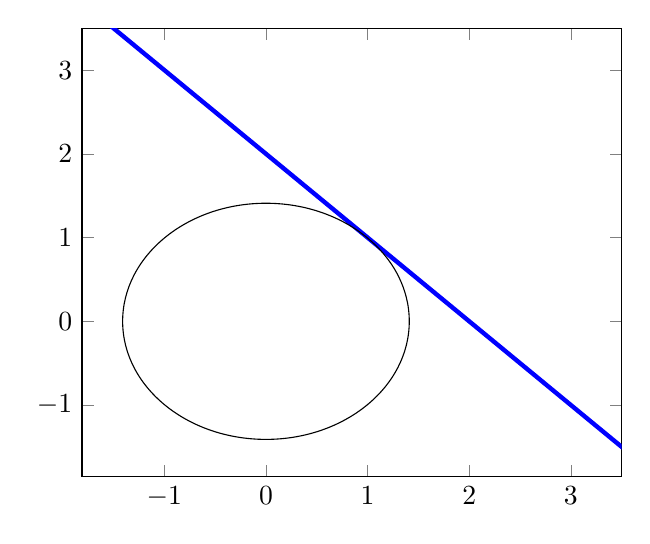
\begin{tikzpicture}
\begin{axis}[xmax=3.5,ymax=3.5, samples=50]
  \addplot[blue, ultra thick] (x,2-x);
  \draw (axis cs:0,0) circle [red, radius=1.41];
\end{axis}
\end{tikzpicture}
    \caption{aaa}\label{aaaa}
  \end{figure}
  La recta $C_1$ interseca al círculo de forma tangencial en el punto $(1,1)$. De hecho si homogenizamos y buscamos las intersecciones de las curvas proyectivas
  \begin{align*}
     & \tilde C_1\:\ x+y=2z,\\
     & \tilde C_2\:\ x^2+y^2=2z^2,
  \end{align*}
  entonces despejamos $z=\frac{x+y}{2}$. Lo que nos lleva a $x^2+y^2=2\left(\frac{x+y}{2}\right)^2$. Despejando vale que $(X-Y)^2=0$ y no podría ocurrir que $X,Y$ son ambos cero y $X=Y$. Esto nos lleva al punto $[X,X,X]=[1,1,1]\in\tilde C_1\cap\tilde C_2$ y este punto corresponde al punto afín que ya habíamos encontrado.\par
  Nosotros esperábamos dos puntos de intersección, pero no hay manera ni siquiera pasando por los complejos. Sólo obtenemos un punto de intersección y esto ocurre porque la recta interseca de manera tangencial. Este problema es el análogo al de una variable, recuerde que el teorema fundamental del álgebra garantiza la existencia cierto número de raíces para los polinomios. Lo que no hemos mencionado es la \emph{multiplicidad} de la raíz. En este caso vemos que la misma ecuación $(X-Y)^2=0$ nos dice que la raíz tiene multiplicidad dos.\par
  En conclusión sólo encontramos un punto de intersección, incluso después de haber buscado posibles puntos en el infinito. Esto es porque $[1,1,1]$ se debe contar con multiplicidad dos y corresponde con el hecho de que ambas curvas se intersecan de manera tangencial en este punto. De hecho, se ve reflejado en que al resolver el sistema de ecuaciones obtuvimos la ecuación $(X-Y)^2=0$.
\end{Ex}

Este no es el único caso en que esto puede ocurrir y el siguiente ejemplo lo ilustra.

\begin{Ex}
  Considere ahora la curvas
  \begin{align*}
     & C_1\:\ y=x,\\
     & C_2\:\ y^2=x^3.
  \end{align*}
    \red{aregar figura} Estas curvas se intersecan en dos puntos del plano afín. Al homogenizar obtenemos
    \begin{align*}
     & \tilde C_1\:\ X-Y=0,\\
     & \tilde C_2\:\ X^3-Y^2Z=0,
  \end{align*}
  y resolviendo llegamos a $X^3-X^2Z=0$ y de aquí que $X=0$ ó $X=Y=Z$. Si $X=0$, entonces $Y=0$ y así $Z$ queda libre lo que nos lleva a los puntos $[1,1,1]$ y $[0,0,1]$. A diferencia del caso anterior, no hay multiplicidades mayores a uno. Aquí lo que ocurre es que uno de los puntos de intersección es un punto que no es suave. Las rectas cuyas direcciones aproximan la identidad tienen dos puntos de intersección con la curva cuspidal, entonces en el límite, el punto singular $[0,0,1]$ tiene multiplicidad dos. \red{agregar figura}
\end{Ex}

\begin{Ex}
  Esta vez consideramos las curvas
  \begin{align*}
     & C_1\:\ x+y+1=0,\\
     & C_2\:\ 2x^2+xy-y^2+4x+y+2=0.
  \end{align*}
  Aquel que esté atento podrá notar que
  $$2x^2+xy-y^2+4x+y+2=(x+y+1)(2x-y+2)$$
  y así $C_1\subseteq C_2$ lo que nos dice que la cantidad de puntos de intersección es infinita. Pero entonces las situaciones así no deben entrar en la consideración de los puntos de intersección de manera tan vaga. En el caso de $\bA^2_\bR$ hay infinitos puntos por lo que debemos especificar lo que buscamos.
\end{Ex}

\begin{Def}
  Sea $C\:\ f(x,y)=0$ una curva con $f\in K[x,y]$. Si factorizamos $f$ como un producto de polinomios irreducibles $f=\prod_{j=1}^{n}p_j$, entonces los \term{componentes} de la curva $C$ son las curvas $C_j\:\ p_j(x,y)=0$. Diremos que $C$ es irreducible cuando tenga un único componente. Es decir, sólo si el polinomio $f$ es irreducible.
\end{Def}

\begin{Ex}
  De las curvas estudiadas en el ejemplo anterior, la curva $C_1$ es irreducible al ser un polinomio lineal y la segunda curva se puede factorizar en dos componentes. Ambas rectas son las componentes irreducibles de esta curva.
\end{Ex}

\begin{Def}
  Diremos que dos curvas afines $C_1, C_2$ no tienen componentes en común si sus componentes irreducibles son distintos.
\end{Def}

Un resultado básico en teoría de curvas que no vamos a demostrar es el siguiente:

\begin{Prop}
  Si $C_1, C_2$ son dos curvas afines sin componentes en común, entonces $C_1\cap C_2$ es un conjunto finito.
\end{Prop}

\begin{Rmk}
  De manera análoga al caso afín, se definen componentes de curvas proyectivas y la noción de dos curvas proyectivas sin componentes comunes.
\end{Rmk}

El teorema de Bezout es más general que este resultado. Con lo que hemos visto hasta ahora, lo podemos enunciar.\red{bajé a agarrar agua}\par
Por ahora mencionamos las siguientes propiedades:
\begin{enumerate}
  \item Si $P\not\in C_1\cap C_2$, entonces $I(C_1\cap C_2,P)=0$.
  \item Si $P\in C_1\cap C_2$ y $P$ es un punto no singular de $C_1$ y $C_2$, y si adicionalmente $C_1$ y $C_2$ tienen direcciones tangenciales diferentes en $P$, entonces $I(C_1\cap C_2,P)=1$. En este caso, se dice que $C_1$ y $C_2$ se intersecan en $P$ de manera transversal.
  \item Si $P\in C_1\cap C_2$ y $C_1$ y $C_2$ no se intersecan transversalmente, entonces $I(C_1\cap C_2,P)\geq 2$.
\end{enumerate}

\begin{Th}[Bezout]
  Sean $C_1,C_2\subseteq\bP_\bC^2$ sin componentes en común. Entonces vale que
  $$\sum_{P\in C_1\cap C_2}I(C_1\cap C_2,P)=\deg(C_1)\deg(C_2).$$
  En particular si $C_1,C_2$ son suaves y únicamente tienen intersecciones transversales, entonces
  $$|C_1\cap C_2|=\deg(C_1)\deg(C_2)$$
  y en todo momento se tiene la desigualdad $|C_1\cap C_2|\leq\deg(C_1)\deg(C_2)$.
\end{Th}

\section{Día n+2| 20210114}

\subsection{Multiplicidad de la intersección de dos curvas}
Vamos a estudiar algunas propiedades y ejemplos de cálculo de la multiplicidad o índice de intersecciones $I(C_1\cap C_2,P)$. Vamos a comenzar con un teorema que establece la existencia de la multiplicidad de la intersección y nos permite hacer cálculos.\par

Rápidamente para poder simplificar la notación introducimos los conceptos de variedad.

\begin{Def}
  La \term{variedad afín} de $f$ es el conjunto de ceros de $f$ dentro del espacio afín $\bA^2$. Denotamos 
  $$V(f)=\set{x\in\bA^2\:\ f(x)=0}$$
  y análogamente la \term{variedad proyectiva} de $F$ es su conjunto de ceros dentro del espacio proyectivo. Este conjunto es
  $$V(F)=\set{X\in\bP^2\:\ F(X)=0}.$$
\end{Def}
\begin{Th}
  Considere $V(f),V(g)$ dos curvas afines en $\bA_\bC^2$ y $P\in\bA_\bC^2$ dado. Entonces existe un número $I(V(f)\cap V(g),P)$ definido de manera única tal que las siguientes propiedades se satisfacen:
  \begin{enumerate}
    \item $I(V(f)\cap V(g),P)\in\bZ_{\geq 0}$, a menos que $P$ esté en un componente común de $V(f),V(g)$ y en ese caso $I(V(f)\cap V(g),P)=\infty$.
    \item $I(V(f)\cap V(g),P)=0$ si y sólo si $P\not\in V(f)\cap V(g)$.
    \item Dos rectas distintas se intersecan con multiplicidad uno en su punto de intersección.
    \item $I(V(f)\cap V(g),P)=I(V(g)\cap V(f),P)$.
    \item Si $f=\prod p_i^{\al_i}$ y $g=\prod q_i^{\bt_i}$, entonces
    $$I(V(f)\cap V(g),P)=\sum_{i,j}\al_i\bt_jI(V(p_i)\cap V(q_j),P).$$
    \item $I(V(f)\cap V(g),P)=I(V(f)\cap V(g+hf),P)$ para $h\in\bC[x,y]$.
 \end{enumerate}
\end{Th}

\begin{Def}
  El número $I(V(f)\cap V(g),P)$ se llama \term{multiplicidad de la intersección} de $V(f)$ y $V(g)$ en $P$.
\end{Def}

\begin{Ex}
  \begin{enumerate}
    \item $x^2$ con $y$
    \item círculo con recta
    \item cuspidal con identidad
  \end{enumerate}
\end{Ex}

\begin{Def}
  Sea $f$ un polinomio con coeficientes en $\bC$ y $P\in V(f)$. La \term{multiplicidad} de $f$ en $P$
\end{Def}

ko cums
%%%%%%%%%%%% Contents end %%%%%%%%%%%%%%%%
\ifx\nextra\undefined
\printindex
\else\fi
\nocite{*}
\bibliographystyle{plain}
\bibliography{bibiTNum}
\end{document} 